\chapter{Mechanical Design}
\label{chap:mech_design}
As pointed out in the previous chapter, the major task of this project was to devise an efficient mechanical
design. Two different designs both based on extension springs were looked into. 
This chapter describes them and the motivation behind choosing the final design to be fabricated.

\section{Design 1}
\subsection*{Energy pumping}
\begin{figure}[!h]
\centering
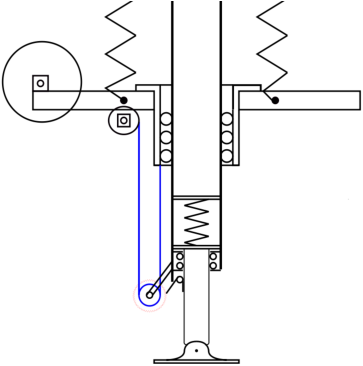
\includegraphics[scale=2]{fig/pratik_des.pdf}
\caption{Winding motor with pulley on the leg}
\label{fig:3_pratik_design}
\end{figure}
Fig. \ref{fig:3_pratik_design} shows the pulley mechanism for storing energy in the large central spring.
The winding motor is placed upon the platform which can be called as the larger mass M of the two mass
system. A winch connects the motor to the same platform passing over the pulley on the lower leg. Thus, as
the motor rotates, it pulls the platform (and itself) downwards while extending the spring above it. 

\subsection*{Constraint}
Fig. \ref{fig:3_pratik_design} also shows the constraint mechanism for the pulley. It consists of a hatch connected to
the lower leg with a torsional spring. The toothed part of the pulley is free to move in the clockwise direction (thus
compressing the torsional spring every time). The lower part of the leg is cylindrical with a top flange which matches
the top face of the cylindrical bushing shown inside the main leg. Thus the lower leg can move only up. The protruding
portion of the main leg prevents the hatch from moving in the clockwise direction, thus constraining the pulley from
rolling back in the anti-clockwise direction.

\subsection*{Using the impact for energy release}
This design is unique because it utilizes the impact force ($m\:v_{touch-down}$) to release the stored energy in the main
spring. Visualize the lower leg impacting on the ground. This results in the hatch (which is holding the pulley from
moving back) impacting against the protrusion of the main leg. Since the impact force is easily larger than the torsional
spring force, the hatch closes and the lower leg goes inside the main leg thus enabling free rotation of the pulley. There
is a compression spring inside the main leg connected to the lower leg which gets compressed while this happens. It is
responsible for pushing the lower leg back outside after $t_{liftoff}$.

\subsection{Evaluation}
\begin{itemize}
\item
The motor has to move a distance twice that of the extension of the spring. This is
especially important when we look at the timescales over which we have to extend the spring, these are around
200-300 msecs. A larger distance in smaller time results in a large $\omega$ for the motor which translates
to a smaller available torque. This necessitates a larger motor that can provide this torque. 
\item
The large mass of the platform (M) is helping in the extension of the spring and hence the torque required
for the winding motor reduces.
\item
It has to be ensured that the winding winch does not slip over the pulley when the platform is suddenly released from
the constraint. At the same time, the winch must be free enough so as not to hinder the movement of the platform after
the release.
\item
The platform moves over the leg with the help of a circular bushing. There is another bushing for the lower leg
to move into the upper leg. These circular bushings are light and durable.
\end{itemize}

\section{Design 2}
\begin{figure}[!h]
\centering
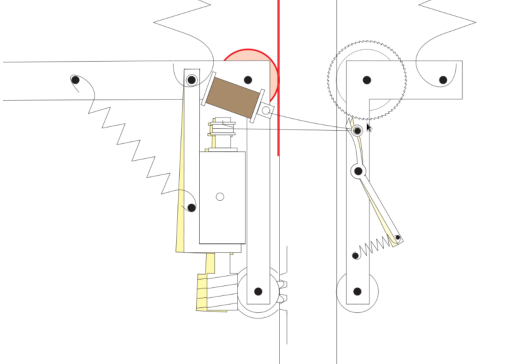
\includegraphics[scale=1.8]{fig/seth_design.pdf}
\caption{Rack and pinion on the leg with the drive motor}
\label{fig:3_seth_design}
\end{figure}

\subsection*{Energy pumping}
Fig. \ref{fig:3_seth_design} shows another design that was considered. The leg consists of a rack on one of its sides. A single dual shaft motor in a sleeve is used to drive the pinion
on this rack as
well as pull the paul to free the ratchet. This motor consists of a string attached to a friction pulley on the shaft.
A friction pulley is a device whose coupling is dependent upon the speed of the relative motion between the two surfaces.
Thus, the motor can pull the paul only beyond a certain $\omega$. Below this speed, the paul spring is strong enough to
engage it with the ratchet. After the paul engages, the string becomes slack again.

\subsection*{Constraint} 
The platform and the ratchet are rigidly connected to a band drive which rolls along
the length of the leg. This ensures that contact of the roller inside the band drive and the leg is maintained at all
times. Since the ratchet is rigidly connected to the platform, both can only move together i.e. only when the paul is
pulled by the drive motor. 

\subsection*{Energy release}
This design uses an electromechanical system to release energy. After sensing the impact through a touch switch located
below the leg, we can use a voice coil actuator to pull the string which in turn moves the paul. This brings in the pull
back spring attached to the sleeve into the picture and it promptly pulls the sleeve away from the rack. Note that the string attached 
to the drive motor pulley is slack at this point.

\subsection{Evaluation}
\begin{itemize}
\item
The sleeve of the motor is kept on the same side as that of the reaction wheel and helps to provide an offset mass for the SLOM effect. The body mass
also helps to obtain an offset C.G.; thus the distance of the reaction wheel from the axis need not as be
as large as calculated in Section \ref{sec:4_rewac}. 
\item
The worm-worm wheel on the rack mechanism provides a huge mechanical advantage and thus reduces the maximum torque required from
the motor. This scales down the mechanical system as well as the electronic system requirements.
\item
All the force of the extension springs is coming as an axial load on the shaft of the motor. We thus
need to choose a gearbox that can handle these axial loads.
\item
The friction pulley has to work against the pual spring, sleeve spring and the horizontal component of the rack force ($k\:x\:tan\:\theta$) to keep the string in tension. This is compounded by the fact that the there is a maximum $\omega$ the motor can
accelerate to in the energy storing phase. It is much better if this $\omega$ is dictated by the torque requirements which are as
critical rather than this mechanism.
\item
Less resolution on the desirable extension of springs because we are operating on a rack. This can however be easily taken care of
in the pitch control law.
\item
The constraint mechanism for Design 2 is not reliable enough and should be improved upon. The major problem is to provide an opposing 
force to the horizontal component of the rack--worm-wheel force ($k\:x\:tan\:\theta$). This force
has to be present when the motor is extending the springs and should be removed before we release the ratchet so that the platform
along with the motor-sleeve is free to move up. To disengage the motor from the rack, the spring shown in the left part of Fig. \ref {fig:3_seth_design} will have to be there as well.
\end{itemize}




